\subsubsection{Pearson}

The pearson product-moment correlation coefficient, or just pearson correlation coefficient, is a way to measure the linear relation, or dependence, between the variables of two sets. This measure can be used to determine the relationship between things like age and blood sugar, height and efficiency in basketball, and how similar people are, based on their taste in media. \cite{Pearson2}

The pearson correlation coefficient creates a linear line of best fit for the two variables, and based on this linear line of best fit, returns a coefficient, which is how much the data of the two variables deviate from this linear line. In Figure \ref{Pearson2} you can see what kind of pattern of data will generate positive, negative, and no correlation using the pearson correlation coefficient. \cite{Pearson2}

\begin{figure}[htb]
\centering
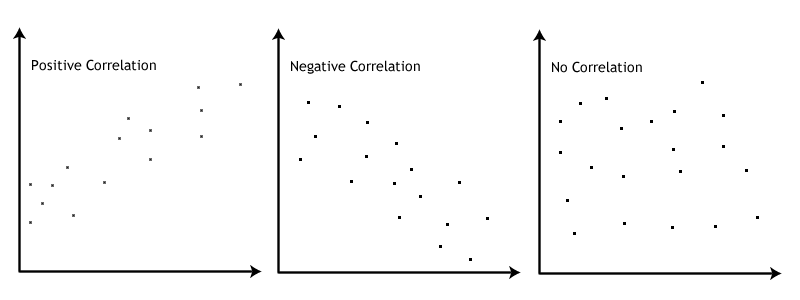
\includegraphics[width=0.8\textwidth]{Images/pearson2.png}
\caption{Showing how two data sets can give differnt Pearson results}
\label{Pearson2}
\end{figure}

The returned coefficient can be in the range of -1 to 1, where -1 is a complete negative relation, 1 is a complete positive relation, and 0 is no relation. Inside this range, there is varying degree of positive and negative relation, with the range of -1 to 0 being negative, and 0 to 1 being positive. This can be seen in Table \ref{PearsonStr}. Pearson very rarely returns perfect relations -1 and 1, and no relation 0. \cite{Pearson2}

\begin{table}[htb]
\centering
\begin{tabular}{|l|l|l|} \hline
	\textbf{Strength} & \textbf{Positive Relation} & \textbf{Negative Relation} \\ \hline
	\textbf{Weak} & 0.1 to 0.3 & -0.1 to -0.3 \\ \hline
	\textbf{Medium} & 0.3 to 0.5 & -0.3 to -0.5 \\ \hline
	\textbf{Strong} & 0.5 to 1 & -0.5 to 1 \\ \hline
\end{tabular}
\caption{Pearons strength scale}
\label{PearsonStr}
\end{table}

In a graph representation, the positive relation would be a linear line going upwards, the negative relation would be a linear line going downwards, and the no relation would be a horizontal line. This can be seen in Figure \ref{Pearson1}. A perfect 1 or -1 relation would be if every point in the graph was placed on the line. \cite{Pearson1}

\begin{figure}[htb]
\centering
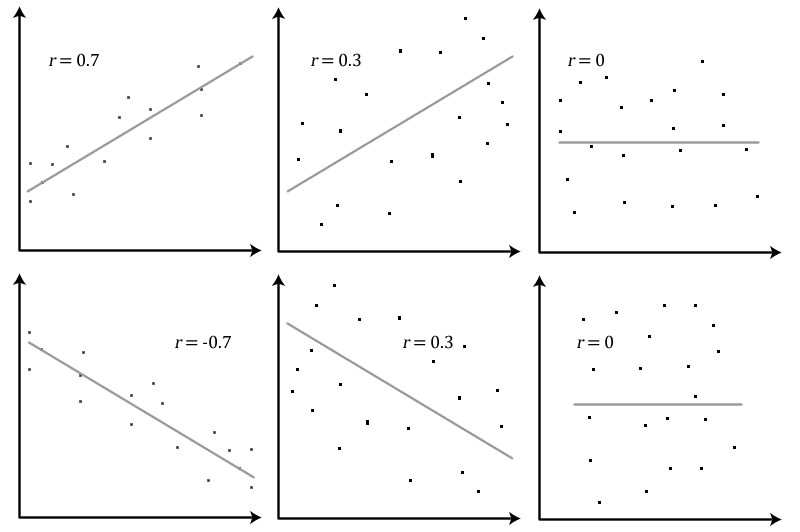
\includegraphics[width=0.8\textwidth]{Images/pearson1.png}
\caption{Showing line representations of data sets, and their correlation}
\label{Pearson1}
\end{figure}

In the context of this project and its possible product, the two variables which would be examined by pearson, is two different people, who uses the product. Pearson would then find the relations between these two people, and use that coefficient as basis for the recommendation process. The data sets it would take in from the two persons, would be the rating they’ve given to the same pieces of media. A point on the graph representation would then be two ratings for the same piece of media. The returned coefficient is then going to be how similar their rating are, and their rating habits. Using the rating given to the media in the product means that pearson is going to supplement the collaborative filtering in the recommendation process.

The calculation to create the pearson correlation coefficient can be seen in Figure \ref{PearsonCalc}. In this calculation, x is the set of ratings from the first person, y is the set of ratings from the second person, n is amount of media items which is examined, and r is the returned pearson correlation coefficient. \cite{Pearson1}

\begin{figure}[htb]
\centering
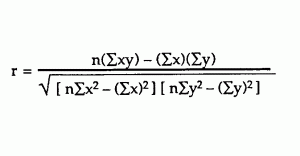
\includegraphics[width=0.5\textwidth]{Images/pearsonCalc.png}
\caption{How the Pearson coefficicent is calculated}
\label{PearsonCalc}
\end{figure}

\subsubsection{Spearman}

Besides the pearson correlation coefficient, it was also considered to use the Spearman’s Rank correlation coefficient, which in many ways works similar to pearson, but has some significant differences. Actually, Spearman is defined as the Pearson correlation coefficient, but between the ranked variables instead, which is a different way to handle the two sets of data. \cite{Spearman2}

\begin{figure}[htb]
\centering
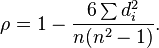
\includegraphics[width=0.4\textwidth]{Images/SpearmanCalc.png}
\caption{How the Spearman coefficient is calculated}
\label{SpearCalc}
\end{figure}

The spearman correlation coefficient starts by finding two ranking lists, one for each of the sets being processed. The highest rank is either assigned to the lowest or the highest variable in each set, depending on if the set is sorted ascending or descending. The same applies to the lowest variable in each set. Every variable pair should then have a respective rank, reflecting their individual position in the sets they came from. Next, to find the d2 variable seen in Figure \ref{SpearCalc}, you find the sum of the difference between all the ranking pairs squared. See Table \ref{SpearmanEx} for an example. In the example, the sum of d2 is 194, n is the sample size of 10, and returns a correlation coefficient of -0.176, which is a low correlation. \cite{Spearman2}

One more thing to note about spearman is that if you have tied rankings, you have to give them the average of the ranks they otherwise would have had, and use a different way more similar to pearson to calculate the coefficient. \cite{Spearman1}

\begin{table}[htb]
\centering
\begin{tabular}{|l|l|l|l|l|l|} \hline
	\textbf{X} & \textbf{Y} & \textbf{X Rank} & \textbf{Y Rank} & \textbf{D1} & \textbf{D2} \\ \hline
	86 & 0 & 1 & 1 & 0 & 0 \\ \hline
	97 & 20 & 2 & 6 & -4 & 16 \\ \hline
	99 & 28 & 3 & 8 & -5 & 25 \\ \hline
	100 & 27 & 4 & 7 & -3 & 9 \\ \hline
	101 & 50 & 5 & 10 & -5 & 25 \\ \hline
	103 & 29 & 6 & 9 & -3 & 9 \\ \hline
	106 & 7 & 7 & 3 & 4 & 16 \\ \hline
	110 & 17 & 8 & 5 & 3 & 9 \\ \hline
	112 & 6 & 9 & 2 & 7 & 49 \\ \hline
	113 & 12 & 10 & 4 & 6 & 36 \\ \hline
\end{tabular}
\caption{Spearman example on the correlation between IQ and amount of TV watched}
\label{SpearmanEx}
\end{table}

The coefficient generated by spearman works on the same scale pearson does, so Table \ref{PearsonStr} can again be referenced for the meanings of the coefficients. The spearman correlations coefficient is based on the monotonic relationship the two sets of data create\cite{Spearman2}. A monotonic relationship is when the graph representation of the data sets is either always rising or always falling, each respectively giving the perfect and negative perfect coefficient. The variable pairs which deviate from this relationship will worsen the coefficient.

\subsubsection{Comparison}

While pearson works on a linear relationship, spearman’s correlation coefficient works on a monotonic relationship. As seen in Figure \ref{Spearman}, the spearman correlation coefficient will return a perfect relation in the case that the monotonic relationship holds. Spearman is also softer, compared to pearson, in a sense, since deviations has less of an impact, which can easily ruin a high scoring coefficient with pearson. In the context of this project, this property doesn’t suit what the algorithm is supposed to find. With spearman, it could return a perfect relation, even when the two users haven’t given the same piece of media the same rating. The figure also shows the pearson correlation coefficient for the same set of data, which returns a strong, but not perfect, positive relation. This makes more sense in this context, as the peoples ratings is similar, but not exactly the same. Also, the algorithm should strive for the highest possible coefficients, and best possible matches, and therefore is spearmans more softer approach not optimal. Because of this pearson was chosen to be used in the project.

\begin{figure}[htb]
\centering
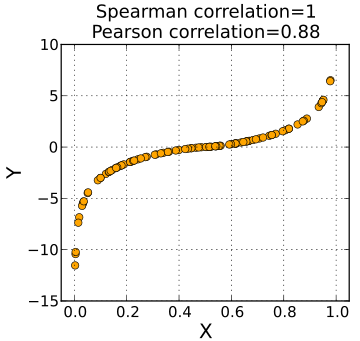
\includegraphics[width=0.6\textwidth]{Images/spearman.png}
\caption{How the Spearmen measure works, compared to Pearson}
\label{Spearman}
\end{figure}

Pearson does have some problems, which can be attributed to the same problems collaborative filtering has. If there is a lack of a suitable large size of data, then pearson can generate inaccurate, and possibly wrong coefficients. For example, if two people have a small number of consumed media in common, small deviations in ratings from each person will have a larger effect on the returned coefficient. It is a problem which will fix itself slowly with time, as more data accumulates and becomes available to the calculation. Also, if there is only two pairs of variables, pearson will never return anything but perfect and no correlation coefficients. Because of this it should be considered to implement a secondary part to the recommendation algorithm, to combat this possible weakness in the collaborative filtering, and work as supplement to the recommendation algorithm.
